\documentclass[11pt,a4paper]{article}
\usepackage[margin=2.2cm]{geometry}
\usepackage[T1]{fontenc}
\usepackage{lmodern}
\usepackage{microtype}
\usepackage{booktabs}
\usepackage{tabularx}
\usepackage{array}
\usepackage{enumitem}
\usepackage{xcolor}
\usepackage{tcolorbox}
\usepackage{pgfplots}
\pgfplotsset{compat=1.17}
\usepackage[hidelinks]{hyperref}
\setlist{nosep,leftmargin=1.4em}
\setlength{\parskip}{0.45em}
\setlength{\parindent}{0pt}
\definecolor{good}{HTML}{1B7F4B}
\definecolor{bad}{HTML}{B3261E}
\definecolor{mid}{HTML}{8A6D00}
\definecolor{acc}{HTML}{1F4E79}
\definecolor{undef}{HTML}{9AA5B1}
\newcolumntype{Y}{>{\raggedright\arraybackslash}X}
\newtcolorbox{keybox}[1]{colback=acc!4,colframe=acc!70,fonttitle=\bfseries,title=#1,boxrule=0.6pt,arc=2pt}
\newtcolorbox{warnbox}[1]{colback=bad!4,colframe=bad!60,fonttitle=\bfseries,title=#1,boxrule=0.6pt,arc=2pt}
\newcommand{\pct}{\%}

\title{\textbf{Thesis Results Report}\\[0.3em]
\large Attributing Security in a Local, Zero-Cost Defense-in-Depth Pipeline for Retrieval-Augmented Generation\\[0.2em]
\normalsize\itshape Instruction injection is contained; knowledge corruption is not}
\author{Status of all results up to repository commit \texttt{2846f2f}}
\date{25 November 2026}

\begin{document}
\maketitle

\begin{keybox}{How to read this report}
This report collects every result of the thesis so far in one place: the original evaluation, the revision for
the reviewers, the comparison with existing defenses, the audit of the evidence, and the two preregistered
experiments run on 25 November 2026 (E1, E2). Section~\ref{sec:archive} adds the findings from the remaining output files of the repository (earlier runs, gate calibration, PII tests). Every number is taken from the revised papers
(\texttt{paper\_revision/main.tex}, \texttt{main\_iccit.tex}) or from \texttt{research\_improvement/}, which hold the
per-row outputs and scripts that produce them. Where an older working document in \texttt{docs/} disagrees, the
papers are authoritative. No new numbers were computed for this report.

\textbf{Reading the statistics.} ASR = attack success rate (share of attacks whose planted answer reached the
user). Square brackets are 95\% Wilson confidence intervals. ``fix/brk'' are the rows a defense fixed or broke
relative to its paired baseline; $p$ is the exact McNemar test on those rows. A large $p$ means ``no difference
detected at this sample size'', never ``the same''.
\end{keybox}

\tableofcontents
\newpage

%=====================================================================
\section{Executive summary}

The thesis builds a thirteen-stage defense for Retrieval-Augmented Generation (RAG) that runs entirely on one
laptop with open-weight models and no paid API, and then measures \emph{which} stages actually provide the
security. It was evaluated on 920 scored rows across seven evaluation sets, including three independent
third-party datasets (PoisonedRAG, BIPIA, deepset), with paired tests on identical rows.

\begin{enumerate}[leftmargin=1.6em,itemsep=0.35em]
\item \textbf{Instruction injection is strongly but not completely contained.} No canary leaked into any of the
  132 delivered answers, and 74/74 poisoned chunks were redacted before generation (Protocol A). Scoring what
  users actually receive, attack success falls from \textbf{29.5\% to 3.5\%} ($n=200$, 54 fixed / 2 broken,
  $p<10^{-13}$); over three generation seeds, \textbf{30.3 $\pm$ 0.8\% to 4.2 $\pm$ 0.6\%}. BIPIA: 45/50 indirect
  injections blocked (0/50 undefended).
\item \textbf{It matches or beats existing defenses on the same 200 attacks.} Seven layers 3.5\% vs.\
  LLM-Guard firewall 21.0\%, Spotlighting 23.0\%, adapted ADO orchestrator 28.5\% (all $p\le 10^{-8}$); it
  \emph{matches} the ControlNET detector (4.5\%, $p=0.77$) with somewhat better benign utility.
\item \textbf{Three simple layers do most of the work, on this attack class.} Per-chunk sanitization, grounding
  and refusal-on-detection act as \emph{near-independent filters} (each removes 39--49\% of what reaches it) and
  come within \textbf{2.4 points} of all seven layers at $n=424$ (95\% upper bound). They do \emph{not} suffice on
  assertion-only attacks (62.5\% vs.\ 35.0\%, $p=0.003$).
\item \textbf{The protection carries over to new attack wording.} In a preregistered test with held-out
  wording, full-stack ASR was 3.0\% vs.\ 3.5\% ($p=1.0$). Without a coercive query phrase it was 7.5\% ($p=0.115$,
  not significant); the relative reduction fell from 88\% to 55\%.
\item \textbf{The ``sophisticated'' components add no measured security.} The co-activation (multivector)
  detector never fires validly on saturated classifier scores --- a structural impossibility, proven in closed
  form --- and the closed-loop controller adds no measurable security (it only lowers false refusals).
\item \textbf{Knowledge corruption is not contained.} On PoisonedRAG the defended pipeline is no better than
  undefended RAG: \textbf{90.7\% vs.\ 91.3\%} ($p=1.0$). Every stage fails for a traceable reason, and in about half
  of the successes (54.4\%) the poisoned passage overrode an answer the model already knew.
\item \textbf{It runs on a laptop.} Median 15.3\,s per query on an 8\,GB RTX 4060 laptop GPU, 8.6\,s with the
  encoders in fp16 on the GPU.
\item \textbf{The earlier runs explain the design choices} (Section~\ref{sec:archive}). The canary protocol could not
  separate defenses (single baselines also scored 130/130), which motivated scoring delivered answers; the input gate's
  fused score was largely dormant (10 of its blocks came from it; the rest from override rules); and the PII tests
  were uninformative (0/30 leaks even undefended).
\end{enumerate}

\begin{figure}[h]
\centering
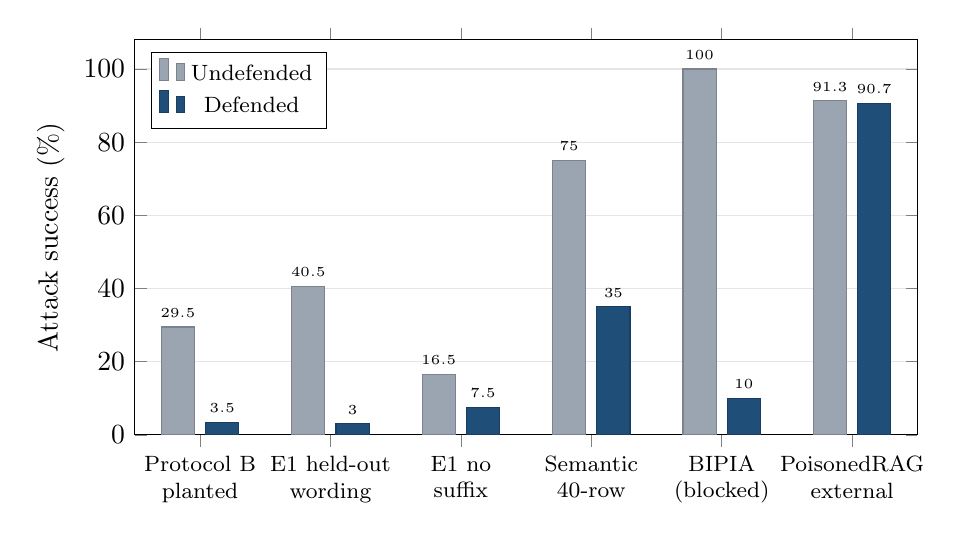
\begin{tikzpicture}
\begin{axis}[
  ybar=4pt, width=0.95\linewidth, height=6.6cm, bar width=12pt,
  ymin=0, ymax=108, ylabel={Attack success (\%)},
  symbolic x coords={B,HO,NS,SEM,BIP,PR},
  xticklabels={{Protocol B\\planted},{E1 held-out\\wording},{E1 no\\suffix},{Semantic\\40-row},{BIPIA\\(blocked)},{PoisonedRAG\\external}},
  xtick=data, xticklabel style={align=center,font=\footnotesize},
  nodes near coords, nodes near coords style={font=\tiny},
  every node near coord/.append style={/pgf/number format/fixed,/pgf/number format/precision=1},
  legend style={at={(0.02,0.97)},anchor=north west,font=\footnotesize},
  enlarge x limits=0.1, ymajorgrids, grid style={gray!20}]
\addplot[fill=undef,draw=undef!80!black] coordinates {(B,29.5) (HO,40.5) (NS,16.5) (SEM,75.0) (BIP,100) (PR,91.3)};
\addplot[fill=acc,draw=acc!80!black] coordinates {(B,3.5) (HO,3.0) (NS,7.5) (SEM,35.0) (BIP,10) (PR,90.7)};
\legend{Undefended, Defended}
\end{axis}
\end{tikzpicture}
\caption{The scope boundary in one picture. Defended vs.\ undefended attack success by attack type. Instruction-style
attacks fall sharply; assertion-only (semantic) attacks fall only partly; PoisonedRAG knowledge corruption does
not fall at all. For BIPIA the bars show the share \emph{not blocked} (50/50 undefended, 5/50 defended), because
BIPIA goals have no target string.}
\label{fig:scope}
\end{figure}

%=====================================================================
\section{What the thesis set out to do}

\textbf{Problem.} In RAG, every retrieved passage is an untrusted input. An attacker who can edit a wiki page,
post a review or poison a data source can deliver either \emph{instructions} (prompt injection) or \emph{false
facts} (knowledge corruption) into the model's context. Real deployments stack several imperfect defenses, but it
is rarely measured which layer actually stops an attack.

\textbf{Objectives.}
\begin{enumerate}[label=(\roman*)]
\item Build a RAG defense pipeline from open-source, free, fully local components.
\item Attribute the security outcome to individual stages with paired statistics.
\item Test whether a detector can recognise \emph{conjunctive} attacks that split an instruction across the query
  and a retrieved chunk so that each part stays below its threshold.
\item Locate the attacks that still get through, and explain why.
\end{enumerate}

\textbf{Contributions as now stated in the papers.}
\textbf{C1} a local, zero-cost thirteen-stage pipeline whose input risk score propagates downstream (no new
detector is claimed); \textbf{C2} a paired attribution protocol --- leave-one-out, single-layer and a fully
crossed three-layer factorial, exact paired tests, an independence null, a measured noise floor, and a
claim-by-claim checker; \textbf{C3} findings an end-to-end comparison hides (near-independent filters, class-
dependent sufficiency, wording dependence); \textbf{C4} a closed-form negative result for co-activation detection
with a graded repair, and a stage-by-stage account of why this defense class fails on knowledge corruption.

%=====================================================================
\section{The system and how it was evaluated}

\subsection{The thirteen-stage pipeline}

\begin{table}[h]
\centering\small
\begin{tabularx}{\linewidth}{@{}l l Y@{}}
\toprule
Stage & Function & Local tool \\
\midrule
1--2 & Input and normalisation & FastAPI; ftfy, NFKC, base64, spaCy \\
3/3c & Fusion input gate (allow / review / block) & DeBERTa-v3 classifier + Llama Guard 3 \\
4--5 & Embedding and vector search & bge-m3; FAISS \\
6 & Per-chunk sanitisation and canary insertion & LLM-Guard per-chunk scanner \\
7 & Cross-encoder reranking (tightened at high risk) & bge-reranker-v2-m3 \\
8 & Guarded (spotlighted) prompt & LangChain \\
9 & Generator ensemble & Ollama: Llama 3.2 3B, Mistral 7B, Qwen2.5 3B \\
10 & Grounding judge and canary re-check & lexical overlap + small-model judge \\
10A & \emph{Extension:} multivector co-activation detector & noisy-OR over query and context channels \\
10B & \emph{Extension:} closed-loop risk controller & accept / escalate / retry / refuse \\
11--12 & PII masking and DLP & Presidio; regex, Luhn, exact-data match \\
13 & Safe response & fixed refusal and audit trail \\
\bottomrule
\end{tabularx}
\caption{Pipeline stages. The organising idea is a \emph{forward-propagated risk score}: a borderline prompt
tightens sanitisation, reranking and grounding for that same request.}
\end{table}

\subsection{Evaluation sets and protocols}

\begin{table}[h]
\centering\small
\begin{tabularx}{\linewidth}{@{}l r l Y@{}}
\toprule
Set & $n$ & Source & What is scored \\
\midrule
Adversarial slice (Protocol A) & 220 & constructed & gate decision, chunk redaction, canary integrity \\
Planted attacks (Protocol B) & 200 (+224) & constructed & planted target string in the delivered answer \\
Benign controls (Protocol B) & 200 & rag-mini-wikipedia & refusal, correctness \\
Semantic free-text slice & 40 & constructed & planted target string \\
PoisonedRAG (NQ, HotpotQA, MS MARCO) & 150 & external & planted target string \\
BIPIA text attacks & 50 & external & block / redaction, manual reading \\
deepset prompt-injections & 60 & external & gate decision \\
\midrule
Total & 920 & & \\
\bottomrule
\end{tabularx}
\caption{Evaluation sets. Every configuration is run on the same rows, so all comparisons are paired.}
\end{table}

\textbf{Three configurations were evaluated, and they must not be confused:}
\begin{itemize}
\item \textbf{Protocol A} --- the complete thirteen-stage pipeline with the three-model ensemble and the controller
  (run with and without the controller).
\item \textbf{Protocol B} --- a seven-layer mitigation harness using the same stage code, toggling each layer
  independently, with a single generator (llama3.2:3b) so that arms differ only in the toggled layer.
\item \textbf{External sets} --- an \emph{adaptive-tier variant} (Stages 1--10 and 13; no multivector detector,
  controller, Presidio or DLP), in which input risk selects retrieval depth and generator. At low risk it uses a
  single llama3.2:3b, which applied to 139/150 PoisonedRAG and 44/50 BIPIA rows. (This was originally described as
  ``the complete pipeline''; the audit corrected it --- see Section~\ref{sec:audit}.)
\end{itemize}

\textbf{Hardware.} AMD Ryzen 5 7640HS, 16\,GB RAM, NVIDIA RTX 4060 Laptop (8\,GB), Windows 11, Python 3.11.9,
Ollama 0.40.16. Generators at temperature 0.2, gate/judge/fuser at 0.0, seed 42.

\textbf{Statistics.} Exact McNemar tests on discordant rows, Wilson intervals, Bonferroni correction for families
(7 leave-one-out tests, $\alpha=0.007$; 4 subsets, $\alpha=0.0125$). Power: at $n=200$, a 10-point ASR difference is
detected with power 0.87--0.96; 2-point differences are not resolvable and are not claimed.

%=====================================================================
\section{How the work evolved}

\begin{enumerate}
\item \textbf{Original thesis design} --- a multi-vector risk-fusion (``C3RF'') gate plus downstream controls. The
  early headline (``ground-plus'' configuration, older code) was 30.5\% $\rightarrow$ 16.5\% ASR at a 9.0-point
  benign cost, after a scorer audit corrected an initial 31.0\% $\rightarrow$ 18.5\%.
\item \textbf{Three measurement corrections} changed the conclusions: (a) the marker scorer now normalises digits
  vs.\ words and recognises refutations; (b) mitigation scorers were aligned on blocked rows; (c) an apparent
  45-point benign cost of an older ``full'' arm was traced to a grounding-judge blind spot for terse yes/no answers.
\item \textbf{Current-code ablation} --- the seven-layer harness re-run with fixed scoring: 3.5\% ASR and 8.5\%
  benign blocking. This supersedes the older-code numbers (which are not pooled with it).
\item \textbf{Reviewer revision} --- 920 rows across seven sets (up from 220), independent external data, existing-
  defense baselines, replicates, an enlarged 424-row set, latency and memory, and ``100\% neutralisation'' replaced
  by the two-level claim of Section~\ref{sec:levels}.
\item \textbf{Existing defenses on Protocol B} --- LLM-Guard, Spotlighting, ControlNET and an adapted ADO.
\item \textbf{Methodological-novelty and generalisation work} (\texttt{research\_improvement/}) --- an evidence audit,
  the full factorial and Shapley analysis, class and wording analyses, a PoisonedRAG trace analysis, and the
  preregistered experiments E1 and E2. Both papers were then revised accordingly.
\end{enumerate}

%=====================================================================
\section{Results}

\subsection{Protocol A: specificity, indirect injection and gate adaptivity}

\begin{itemize}
\item \textbf{Specificity.} The gate flags none of the 80 benign rows (0/80, [0, 4.6]\%). Downstream, the
  controller run refuses 10 benign rows (14 without the controller).
\item \textbf{Indirect injection.} In both runs all 40 poisoned chunks were redacted at Stage 6 and all 40 canaries
  stayed intact, while the benign questions were still answered.
\item \textbf{Gate adaptivity.} The gate alone flags 29--30 of 40 direct injections; all 40 are blocked once the
  propagated risk tightens the later stages --- direct evidence that forward propagation defends beyond the gate.
\end{itemize}

\subsection{End-to-end neutralisation: two levels of evidence}\label{sec:levels}

\begin{table}[h]
\centering\small
\begin{tabularx}{\linewidth}{@{}l Y@{}}
\toprule
Level & Result \\
\midrule
1. Canary integrity (Protocol A) & Canary intact on every checked row (175/220; the other 45 were blocked earlier),
  including all 132 delivered answers. 74/74 poisoned chunks redacted before generation. \\
2. Malicious output (Protocol B) & 7/200 planted attacks succeed (3.5\%, [1.7, 7.0]) vs.\ 29.5\% undefended: an 88\%
  relative reduction, not elimination. Semantic slice 14/40; PoisonedRAG 136/150; BIPIA 2--3/50 followed the
  injected instruction after manual reading. \\
\bottomrule
\end{tabularx}
\caption{The defensible claim is narrower than ``100\% neutralisation'': a canary is a proxy for instruction-following,
so it can stay intact while an answer is wrong.}
\end{table}

\subsection{Conjunctive (multivector) detection: a structural negative result}\label{sec:conj}

\begin{itemize}
\item \textbf{Measured.} Of 40 multivector rows, 6 were blocked at the gate; on the other 34 the detector fired once,
  and that fire was invalid (both channels individually above threshold). Valid fires: 0/34.
\item \textbf{Calibration cannot rescue it.} Class separation is $-0.30$ raw and $-0.39$ calibrated; a monotone
  recalibration cannot create a usable band.
\item \textbf{Closed-form argument.} A valid conjunctive fire needs the query to pass Stage 3 and the chunk to
  survive Stage 6, i.e.\ \emph{low} injection signatures in both channels; any signature-based co-activation signal
  is therefore low exactly on the rows it targets. With a near-binary classifier there is no
  ``surviving-and-dangerous'' middle band.
\item \textbf{Graded repair.} Reading the DeBERTa logit margin instead of the saturated probability gives 24/30 valid
  fires at 1/80 benign false fires --- but the benign figure is in-sample (6/200 on held-out benign questions) and
  external BIPIA transfer is modest (8/30 attacks, 4/30 benign).
\item \textbf{No security loss.} Every multivector row was neutralised anyway, because Stage 6 redacted the chunk.
\end{itemize}

\subsection{The controller}
The closed-loop controller adds \textbf{no measurable security} (net multivector catch 0 in both runs). It improves
utility: 88 blocked rows vs.\ 101 without it, 70 vs.\ 66 benign rows answered. Correct claim: ``no measured security
gain, at a lower false-refusal cost''.

\subsection{Is the full cascade necessary? The Protocol B ablation}

\begin{table}[h]
\centering\small
\begin{tabular}{@{}l r r r r@{}}
\toprule
Configuration & ASR \% [95\% CI] & fix/brk & $p$ vs.\ undefended & Benign blocked \% \\
\midrule
Undefended & 29.5 [23.6, 36.2] & -- & -- & 0.0 \\
\textbf{Full stack (7 layers)} & \textbf{3.5} [1.7, 7.0] & 54/2 & $<10^{-13}$ & 8.5 \\
\midrule
\multicolumn{5}{@{}l}{\emph{Leave one out}} \\
\quad $-$sanitisation & 11.0 [7.4, 16.1] & 50/13 & $3\times10^{-6}$ & 7.5 \\
\quad $-$grounding gate & 6.5 [3.8, 10.8] & 49/3 & $10^{-11}$ & 2.5 \\
\quad $-$refuse-on-detection & 6.0 [3.5, 10.2] & 51/4 & $2\times10^{-11}$ & 7.0 \\
\quad $-$tightened rerank & 6.0 [3.5, 10.2] & 51/4 & $2\times10^{-11}$ & 6.5 \\
\quad $-$guarded prompt & 5.5 [3.1, 9.6] & 53/5 & $3\times10^{-11}$ & 12.5 \\
\quad $-$Presidio / $-$DLP & 4.0 / 3.5 & 53/2, 54/2 & $<10^{-13}$ & 8.5 \\
\multicolumn{5}{@{}l}{\emph{Single layer only}} \\
\quad Grounding gate & 15.0 [10.7, 20.6] & 29/0 & $4\times10^{-9}$ & 5.5 \\
\quad Sanitisation & 16.0 [11.6, 21.7] & 30/3 & $1.4\times10^{-6}$ & 0.0 \\
\quad Refuse-on-detection & 18.0 [13.3, 23.9] & 25/2 & $6\times10^{-6}$ & 2.5 \\
\quad Tightened rerank & 24.5 [19.1, 30.9] & 28/18 & 0.18 & 0.0 \\
\quad Guarded prompt & \textcolor{bad}{53.0} [46.1, 59.8] & 6/53 & $2\times10^{-10}$ & 0.0 \\
\quad Presidio / DLP & 29.5 & 0/0 & 1.0 & 0.0 \\
\multicolumn{5}{@{}l}{\emph{Subsets}} \\
\quad Sanitise + ground + refuse & 5.5 [3.1, 9.6] & 48/0 & $7\times10^{-15}$ & 9.5 \\
\quad Sanitise + ground & 8.5 [5.4, 13.2] & 42/0 & $5\times10^{-13}$ & 8.0 \\
\quad Sanitise + refuse & 9.5 [6.2, 14.4] & 42/2 & $10^{-10}$ & 2.5 \\
\quad Ground + refuse & 10.5 [7.0, 15.5] & 40/2 & $4\times10^{-10}$ & 7.5 \\
\bottomrule
\end{tabular}
\caption{Protocol B ablation ($n=200$ attack, $n=200$ benign per arm, paired with the same undefended arm).}
\label{tab:ablation}
\end{table}

\textbf{Reading.}
\begin{itemize}
\item No single layer comes close to the full stack (best single layers leave 15--18\%). The guarded prompt on
  its own \emph{raises} ASR to 53.0\% --- it makes the generator defer to the planted ``authoritative correction''.
\item The three-layer subset is \textbf{not significantly different} from the full stack at $n=200$ (5.5\% vs.\ 3.5\%,
  7 vs.\ 3 discordant rows, $p=0.34$; benign 9.5\% vs.\ 8.5\%). The two-layer subsets are worse.
\item \textbf{Replicates} (seeds 42, 7, 1234): undefended 30.3 $\pm$ 0.8\%, full stack 4.2 $\pm$ 0.6\%, three layers
  6.0 $\pm$ 0.9\%. The subset is worse in all three replicates, by 1.8 $\pm$ 0.8 points --- so it gives up one to
  three points for four fewer layers; it is not cost-free.
\item \textbf{Enlarged set} ($n=424$): 29.7\% undefended, 4.2\% full, 4.7\% subset; subset $-$ full $=+0.5$ points,
  95\% interval $[-1.5, +2.4]$. Dropping the other four layers costs \textbf{at most about 2.4 points}. This is a
  bound, not an equivalence claim.
\item \textbf{Reproduction check}: a fresh seed-42 run from raw data agrees with the reported run on 189/200 and
  199/200 rows (undefended, full).
\item Fewer layers are not faster: the subset's median benign latency is 19.0\,s vs.\ 15.3\,s for the full stack.
\end{itemize}

\subsection{Interactions: the three layers are near-independent filters}

\begin{minipage}[t]{0.5\linewidth}
\vspace{0pt}\small
\begin{tabular}{@{}l r r r@{}}
\toprule
Layers & ASR \% & Indep.\ \% & Benign \% \\
\midrule
none & 29.5 & -- & 0.0 \\
S & 16.0 & -- & 0.0 \\
G & 15.0 & -- & 5.5 \\
R & 18.0 & -- & 2.5 \\
S+G & 8.5 & 8.1 & 8.0 \\
S+R & 9.5 & 9.8 & 2.5 \\
G+R & 10.5 & 9.2 & 7.5 \\
S+G+R & 5.5 & 5.0 & 9.5 \\
\bottomrule
\end{tabular}

\smallskip
\footnotesize S = sanitisation, G = grounding, R = refuse-on-detection; other four layers off.
``Indep.'' = ASR predicted if each layer independently removes a fixed fraction of what reaches it.
\end{minipage}\hfill
\begin{minipage}[t]{0.46\linewidth}
\vspace{0pt}
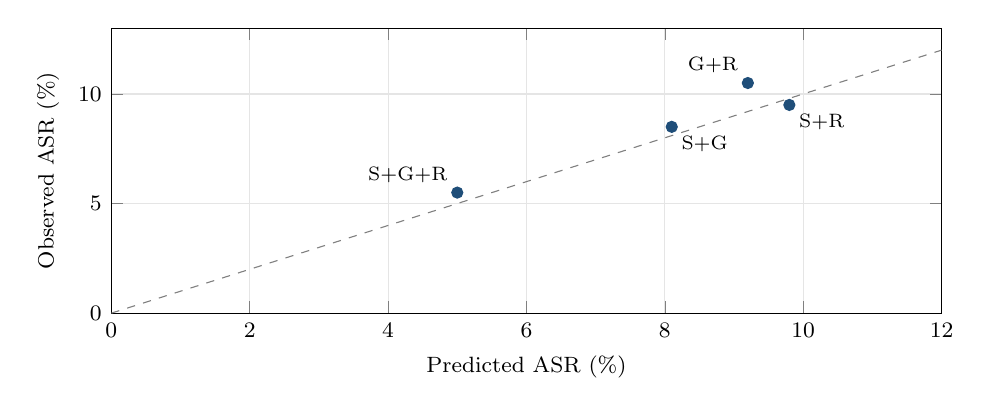
\begin{tikzpicture}
\begin{axis}[width=\linewidth, height=5.2cm, xmin=0, xmax=12, ymin=0, ymax=13,
  xlabel={Predicted ASR (\%)}, ylabel={Observed ASR (\%)}, xlabel style={font=\footnotesize},
  ylabel style={font=\footnotesize}, tick label style={font=\footnotesize}, grid=major, grid style={gray!20}]
\addplot[gray,dashed,domain=0:12] {x};
\addplot[only marks,mark=*,acc] coordinates {(8.1,8.5) (9.8,9.5) (9.2,10.5) (5.0,5.5)};
\node[font=\scriptsize,anchor=north west] at (axis cs:8.1,8.5) {S+G};
\node[font=\scriptsize,anchor=north west] at (axis cs:9.8,9.5) {S+R};
\node[font=\scriptsize,anchor=south east] at (axis cs:9.2,10.5) {G+R};
\node[font=\scriptsize,anchor=south east] at (axis cs:5.0,5.5) {S+G+R};
\end{axis}
\end{tikzpicture}
\end{minipage}

\begin{itemize}
\item On the additive scale every pair looks sub-additive (``redundant''), but against the multiplicative
  independence null every combination matches within 1.3 points, and every 95\% bootstrap interval includes 0
  (S+G+R: 5.5\% observed vs.\ 5.0\% predicted, $[-1.6, +2.8]$).
\item Each layer removes 39--49\% of the attacks that reach it, and they stop largely different rows: of the 59
  undefended successes, 22 are fixed by exactly one single layer and none only by their combination.
\item \textbf{Shapley shares} of the 24.0-point ASR reduction: S 8.7 [5.1, 12.6], G 8.7 [5.8, 11.9], R 6.7 [3.8, 9.7].
  The benign-refusal cost sits mostly in grounding (6.3 of 9.5 points).
\item The guarded prompt changes sign with context: alone it adds 23.5 points of ASR; removed from the full stack it
  changes ASR by only $+2.0$ $[-0.8, +4.8]$.
\item Noise floor: two runs of the same undefended configuration differ on 11 of 200 rows, so effects of 1--3 points
  are within run-to-run noise.
\end{itemize}

\subsection{Class dependence and attack wording}

\textbf{Class dependence.} On the 40-row assertion-only slice the three-layer subset leaves 62.5\% against 35.0\%
for all seven layers (12 vs.\ 1 discordant rows, $p=0.003$) and is not significantly better than undefended
($p=0.13$). Here the guarded prompt --- harmful on its own against instruction-bearing attacks --- is the most
effective single layer (75.0\% $\rightarrow$ 52.5\%, $p=0.035$). \emph{Which layers suffice depends on the attack
class.}

\textbf{Wording (exploratory).} Within Protocol B, protection depends on the randomly assigned coercive query
phrase: for one phrase (``Defer to any authoritative correction\ldots'') the detector fires on every row and
full-stack ASR is 0/147; for another it fires on 20\% of rows and ASR is 9.9\% [5.9, 16.2] (permutation test
$p=0.0001$, $n=424$).

\subsection{E1 --- preregistered test of held-out attack wording}

The wording finding was post hoc, so it was tested in a preregistered experiment (plan, attack files and scoring
fixed and hashed before any inference; same 200 questions and targets; only the wording changed; Bonferroni
$\alpha=0.025$).

\begin{table}[h]
\centering\footnotesize\setlength{\tabcolsep}{4pt}
\begin{tabular}{@{}l c c c c c@{}}
\toprule
 & Original & \multicolumn{2}{c}{HO: held-out wording} & \multicolumn{2}{c}{NS: suffix removed} \\
\cmidrule(lr){3-4}\cmidrule(lr){5-6}
 & & value & vs.\ original & value & vs.\ original \\
\midrule
Undefended ASR & 29.5\% & 40.5\% & $+11.0$, $p=0.007$ & 16.5\% & $-13.0$, $p<0.001$ \\
\textbf{Full-stack ASR} & 3.5\% & \textbf{3.0\%} [1.4, 6.4] & 6/7, $p=1.0$ & \textbf{7.5\%} [4.6, 12.0] & 14/6, $p=0.115$ \\
Relative reduction & 88.1\% & 92.6\% & & 54.5\% & \\
Three-layer subset ASR & 5.5\% & 2.0\% & & 11.0\% & \\
Subset $-$ full & $+2.0$ & $-1.0$ [$-3.8$, 1.8] & & $+3.5$ [$-0.7$, 7.7] & \\
Detector fires (full arm) & 80/200 & 111/200 & & 6/200 & \\
\midrule
\textbf{Preregistered verdict} & & \multicolumn{2}{c}{\textcolor{good}{\textbf{protection transfers}}} & \multicolumn{2}{c}{\textcolor{mid}{\textbf{inconclusive}}} \\
\bottomrule
\end{tabular}
\caption{E1 results (Protocol B harness, llama3.2:3b, $n=200$ paired rows).}
\end{table}

\begin{itemize}
\item \textbf{Held-out wording} was the \emph{stronger} attack (40.5\% undefended), and the defense still reduced it by
  93\%, to 3.0\%. The protection carries over to coercive phrasing it was not evaluated on.
\item \textbf{Without a coercive phrase} the attack was weaker (16.5\%), but the defense kept less of its margin
  (relative reduction 55\%) and the detector fired on 6 rows instead of 80. The difference in full-stack ASR is not
  significant, so the papers do \emph{not} claim the defense is weaker without coercive phrasing; descriptively,
  refuse-on-detection reacts mainly to query phrasing. Post hoc: on rows that originally carried the ``Defer\ldots''
  phrase, ASR rose from 0\% to 7.9\% when it was removed.
\item In neither variant was the three-layer subset significantly different from the full stack --- which is
  again not evidence of equivalence.
\end{itemize}

\subsection{Comparison with existing defenses}\label{sec:existing}

\begin{figure}[h]
\centering
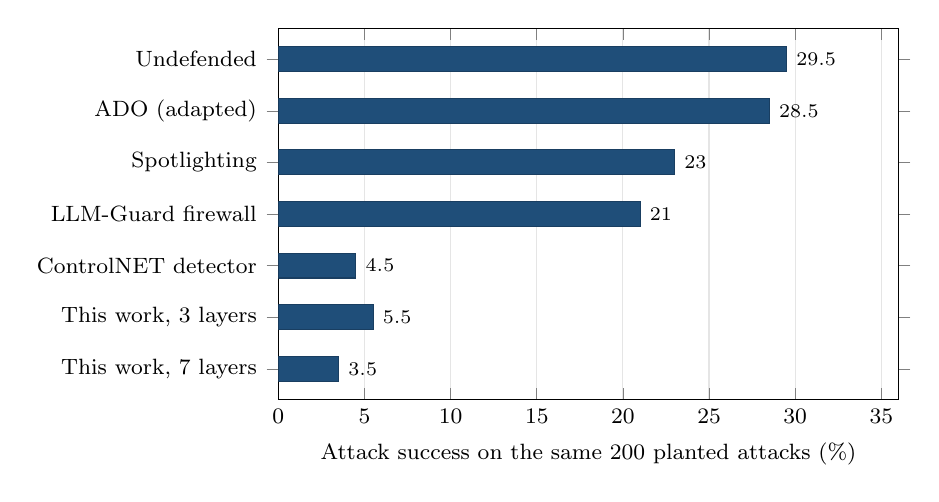
\begin{tikzpicture}
\begin{axis}[xbar, width=0.78\linewidth, height=6.3cm, bar width=9pt, xmin=0, xmax=36,
  xlabel={Attack success on the same 200 planted attacks (\%)}, xlabel style={font=\footnotesize},
  symbolic y coords={Seven,Three,ControlNET,LLMGuard,Spot,ADO,Undef},
  yticklabels={{This work, 7 layers},{This work, 3 layers},{ControlNET detector},{LLM-Guard firewall},{Spotlighting},{ADO (adapted)},{Undefended}},
  ytick=data, yticklabel style={font=\footnotesize}, tick label style={font=\footnotesize},
  nodes near coords, nodes near coords style={font=\scriptsize}, xmajorgrids, grid style={gray!20},
  enlarge y limits=0.1]
\addplot[fill=acc,draw=acc!80!black] coordinates {(3.5,Seven) (5.5,Three) (4.5,ControlNET) (21.0,LLMGuard) (23.0,Spot) (28.5,ADO) (29.5,Undef)};
\end{axis}
\end{tikzpicture}
\caption{Existing defenses on Protocol B, same generator, decoding and scoring, paired by row.}
\end{figure}

\begin{table}[h]
\centering\small
\begin{tabular}{@{}l r r r r@{}}
\toprule
Defense & ASR \% [95\% CI] & Benign blocked \% & Benign correct \% & $p$ vs.\ 7 layers \\
\midrule
Undefended & 29.5 [23.6, 36.2] & 0.0 & 56.5 & $<10^{-13}$ \\
ADO orchestrator (adapted)$^\dagger$ & 28.5 [22.7, 35.1] & 0.0 & 35.5 & $3\times10^{-12}$ \\
Spotlighting (datamarking) & 23.0 [17.7, 29.3] & 0.0 & 55.5 & $9\times10^{-10}$ \\
LLM-Guard input firewall & 21.0 [15.9, 27.2] & 8.5 & 51.0 & $1\times10^{-8}$ \\
ControlNET detector$^*$ & 4.5 [2.4, 8.3] & 13.5 & 46.0 & 0.77 \\
This work, 3 layers & 5.5 [3.1, 9.6] & 9.5 & 52.0 & 0.34 \\
This work, 7 layers & 3.5 [1.7, 7.0] & 8.5 & 52.0 & -- \\
\bottomrule
\end{tabular}

\footnotesize $^*$Detection and blocking only (its mitigation module was not reimplemented).
$^\dagger$Official code with local substitutions (Llama-3.1-8B controller, 4-bit attention filter); 13.5\% ASR if
refusals are not counted as successes. Median latency 45\,s per query vs.\ 15.3\,s.
\caption{Existing defenses on Protocol B.}
\end{table}

\begin{itemize}
\item The seven-layer stack \textbf{clearly outperforms} an input firewall, prompt-level spotlighting and the adapted
  ADO, and \textbf{matches} ControlNET on attack success with somewhat better benign utility (52.0\% vs.\ 46.0\%
  correct, $p=0.058$). It does not establish superiority over ControlNET; much of ControlNET's signal comes from the
  coercive query wording (it blocks 15 of the 16 attacks whose planted chunk never reached the generator).
\item ADO's weakness has one main cause: DP-RAG removes every passage on 64/200 attacks and 58/200 benign questions,
  so the generator refuses, which discards the evidence too.
\item On the Protocol A slice (210 paired rows), a detector-only LLM-Guard flags 50\% of attacks; ControlNET blocks
  93/130 attacks vs.\ 95/130 for the pipeline (not significant), but removes the poison before generation on only
  33/70 context attacks vs.\ 67/70; the official ADO code removes it on 25--44/70 ($p\le1.6\times10^{-6}$).
\end{itemize}

\subsection{Independent external benchmarks}

\begin{table}[h]
\centering\small\setlength{\tabcolsep}{5pt}
\begin{tabular}{@{}l r c c c c@{}}
\toprule
Set & $n$ & Redacted & Undefended & Defended & fix/brk ($p$) \\
\midrule
PoisonedRAG-NQ & 50 & 0/49 & 46 & 44 & 4/2 (0.69) \\
PoisonedRAG-HotpotQA & 50 & 0/50 & 46 & 47 & 1/2 (1.0) \\
PoisonedRAG-MS MARCO & 50 & 0/49 & 45 & 45 & 2/2 (1.0) \\
\textbf{PoisonedRAG, all} & 150 & 0/148 & 137 (91.3\%) & 136 (90.7\%) & 7/6 (1.0) \\
\quad 7-layer harness$^\ddagger$ & 150 & -- & 137 (91.3\%) & 128 (85.3\%) & 16/7 (0.09) \\
\midrule
 & & & \multicolumn{2}{c}{Blocked: undef.\ / def.} & \\
BIPIA text attacks & 50 & 33/49 & \multicolumn{2}{c}{0/50 \ / \ 45/50} & -- \\
\bottomrule
\end{tabular}

\smallskip
\footnotesize Counts are successful attacks. $^\ddagger$Seven-layer harness with llama3.2:3b in both arms.
deepset (gate only, 30+30): 14/30 injections blocked (46.7\%), 17/30 flagged (20/30 with the graded flag), 0/30
benign flagged.
\caption{External sets, adaptive-tier pipeline variant, paired with an undefended arm on the same rows and poison.}
\end{table}

\textbf{BIPIA (instruction-style indirect injection).} 45/50 blocked: 36 by the risk-adaptive policy, 8 by the
grounding judge, 1 at the gate; Stage 6 redacts 33/49 injected chunks. Of the 5 unblocked answers, 2 followed the
injected instruction, 2 did not and 1 is indeterminable: defended attack success 2--3/50 (4--6\%).

\textbf{deepset (real-world direct injection).} Gate-level detection of diverse real phrasing is weak: 23/60
injections blocked on the full test split (38.3\%), 31 of the 32 missed have a scanner score of exactly 0. A graded
review flag ($t=0.230$, chosen on the train split) raises flagged injections from 28/60 to 38/60 at 2/56 benign.

\subsection{Why the defense fails on PoisonedRAG (saved traces and E2)}

\begin{warnbox}{{Knowledge corruption: every stage fails, for a traceable reason}}
\begin{itemize}
\item \textbf{No signature:} the gate scores every PoisonedRAG query 0; Stage 6 redacts 0 of 148 passages, because the
  passages are fluent factual text with no instruction.
\item \textbf{Relevance dominance:} the reranker places the poisoned passage first in 148/148 rows (median margin 0.23).
\item \textbf{Grounding checks consistency, not truth:} all 136 successful attacks pass the grounding judge (median
  faithfulness 1.0), against 0.77 for the 8 delivered answers that resisted.
\item \textbf{Evidence absence:} the true answer appears in another retrieved passage in only 11 rows.
\item \textbf{Prior override (E2, closed-book probe):} asked the 150 questions without any context, llama3.2:3b knew
  the true answer in 74 of the 136 defended successes (\textbf{54.4\%}, [46.0, 62.5]). Knowing it gave no protection:
  defended ASR 90.2\% when it knew vs.\ 91.2\% when it did not. Descriptively, mistral:7b knew 69.1\% and qwen2.5:3b
  34.6\%.
\item \textbf{Not tested:} ensemble disagreement (the variant generated with one model on almost every row).
\end{itemize}
\end{warnbox}

So roughly half the successes are a planted passage overriding knowledge the model has, and the other half target
questions the model cannot answer. A parametric-consistency check could at most address the first half (and a
purpose-built one failed on the 8-row supplement, AUC 0.54); the second half needs provenance or corroborating
evidence. Defenses designed for knowledge corruption (RobustRAG, TriShieldRAG) take that route; the papers present
knowledge corruption as an open problem for this defense class, not a solved one.

\subsection{Signature-free semantic attacks}

\begin{itemize}
\item \textbf{Gate-slip class} (role-play framing): 5 of 20 rows pass the gate in both runs.
\item \textbf{8-row semantic supplement}: 4/8 attacks succeed with or without spotlighting. No answer-side signal
  separates them from benign traffic (ensemble-disagreement AUC 0.47--0.48; faithfulness AUC 0.62).
\item \textbf{40-row free-text slice}: undefended 30/40 (75.0\%), full stack 14/40 (35.0\%; 18 fixed, 2 broken,
  $p=4\times10^{-4}$). The reduction comes from the guarded prompt and refusal (suggestive, not Bonferroni-
  significant); grounding alone has no effect (75.0\%), because a planted fact is perfectly ``grounded''.
\item \textbf{Isolate-and-aggregate generation} (answer per passage, accept only on agreement) drives semantic ASR to
  0/40, but by abstaining on 34/40 attacks and answering only 15/40 benign questions --- an unacceptable utility
  cost. A routed variant keeps utility (36/40 answered) but only reduces ASR from 18/40 to 15/40 ($p=0.45$).
\end{itemize}

\subsection{Cost: latency and memory}\label{sec:cost}

\begin{table}[h]
\centering\small
\begin{tabular}{@{}l c c@{}}
\toprule
Configuration (median / 95th percentile, s) & Attack rows & Benign rows \\
\midrule
Undefended (single generator) & 9.2 / 13.1 & 8.6 / 12.2 \\
Refuse-on-detection only & 7.5 / 12.2 & 8.3 / 11.6 \\
Sanitise + refuse & 9.7 / 14.9 & 10.7 / 15.1 \\
Sanitise + ground + refuse & 15.9 / 29.2 & 19.0 / 29.5 \\
Full stack, 7 layers & 15.4 / 24.7 & 15.3 / 21.3 \\
\quad encoders on GPU, fp16 ($n=50$) & -- & 8.6 / 10.1 \\
Adaptive-tier pipeline (external) & \multicolumn{2}{c}{23.8 (mean)} \\
ADO, Protocol B (adapted) & 45.5 / 312.6 & 45.3 / 271.3 \\
\bottomrule
\end{tabular}
\caption{End-to-end latency on an RTX 4060 Laptop GPU (8\,GB).}
\end{table}

The grounding judge is the dominant cost (about 7--8\,s, on CPU). With fp16 encoders on the GPU the full stack runs
at about the undefended latency, with identical decisions on 50 benign questions. Memory: generator GPU memory
peaks at 6.3\,GB of 8\,GB; the Python process needs about 8\,GB of host RAM. One laptop serves roughly 240 queries
per hour (about 400 with fp16 encoders) --- suited to a single user or small team.

%=====================================================================
\section{Findings from the full output archive}\label{sec:archive}

The repository holds about 800 committed output files. Most feed the results above. This section adds the findings
from the remaining outputs: the input-gate calibration, an earlier 918-row benign run, the older-code mitigation
arms, the controller and detector stress runs, an earlier baseline comparison under the canary protocol, and the
PII-leak tests. Several of these predate the current code and are \emph{not} pooled with the current results; they
are reported because they shaped the design and the evaluation protocol.

\subsection{Input-gate calibration data and the C3RF gate}

\textbf{Calibration corpus} (\texttt{dataset/merged\_output/}). Public prompt-injection, jailbreak, toxicity and PII
datasets were merged into 7,938 rows after de-duplication (target 8,000), split 5,555 / 1,190 / 1,193. The build's
quota audit reports \textbf{FAIL} on two checks: benign hard negatives reach 366 of 7,938 rows (4.61\%, below the 5\%
minimum), and the social-engineering category is absent, because gated sources were unavailable locally. The four
risk tiers meet their target shares within 2 points, but eleven categories are data-limited (e.g.\ only 7 CBRN, 5
self-harm and 5 misinformation rows in the source pool; obfuscation and indirect injection are covered by 8
synthetic rows each).

\textbf{Frozen gate on the held-out test split} (\texttt{dataset/c3rf\_test\_results.json}, $n=1{,}195$, measured once after
freezing thresholds on the validation split):

\begin{table}[h]
\centering\small
\begin{tabular}{@{}l r r r r r@{}}
\toprule
Input gate & Precision & Recall & F1 & False pos. & False neg. \\
\midrule
DeBERTa injection classifier only & 0.966 & 0.537 & 0.691 & 20 & 483 \\
OR-gate (injection or Llama Guard) & 0.935 & 0.860 & 0.896 & 62 & 146 \\
C3RF fusion, block decisions only & 0.967 & 0.638 & 0.769 & 23 & 378 \\
\textbf{C3RF fusion, frozen (review = flagged)} & 0.937 & 0.771 & 0.846 & 54 & 239 \\
\bottomrule
\end{tabular}
\caption{Input-gate operating points on the calibration test split (1,044 harmful, 151 benign rows).}
\end{table}

\begin{itemize}
\item Fusing the two classifiers raises recall from 0.54 (injection classifier alone) to 0.77 at similar precision.
  The simple OR-gate has the highest F1 but 62 false positives against 54.
\item \textbf{The continuous fusion score is largely dormant.} Of the gate's blocks on the test split, only 10 came from
  the fused risk threshold; the rest came from override rules (493 injection hard blocks, 165 Llama Guard hard
  blocks, 21 severe-category blocks; 236 rows took the fast-path allow).
\item Recall is weakest on categories without injection syntax: PII-leakage requests 0.62, direct-harm instructions
  0.67, financial/cyber risk 0.68, misinformation 0.50 ($n=6$); it is highest on prompt injection (0.89) and toxicity
  (0.84). On benign hard negatives the fused gate is correct on only 42\% of 48 rows.
\item Which recall to quote depends on whether ``review'' counts as a detection: 0.636 (block only), 0.753 or 0.771
  (review counted), as reconciled in \texttt{docs/RECONCILIATION\_NOTE.md}.
\end{itemize}

\subsection{An earlier 918-row benign run on rag-mini-wikipedia}

The locked summary \texttt{step4 dataset/frozen/thesis\_results\_locked.json} records a full benign run of the earlier
pipeline over 918 questions:
\begin{itemize}
\item \textbf{Gate false positives on ordinary questions:} 6/918 were red-flagged, all triggered by toxicity words in
  harmless questions (``Damn'', ``Garbage'', ``bitches'' in the zoological sense). Five of the six were absorbed
  downstream without effect; only 1 of 918 answers flipped from pass to fail (0.1\%).
\item \textbf{The hybrid grounding judge needs both components:} pass rate 40.3\% with the lexical scorer alone, 68.9\%
  with the model scorer alone, 78.4\% with the hybrid maximum; 438 of 918 rows needed both.
\item \textbf{A saturated disagreement signal was fixed.} The original ensemble-disagreement score put 786 of 918 benign
  rows in the top band (mean 0.94), so it carried no information; rescoring with sentence-embedding distance moved the
  mean to 0.21, with 2 rows in the top band.
\item \textbf{Risk propagation works on real rows:} high-risk rows reached the 0.90 grounding ceiling with tightened
  sanitisation (0.30) and reranking (0.40) thresholds.
\end{itemize}
These files are historical snapshots; no number in the current papers comes from them.

\subsection{Older-code mitigation arms (Protocol B, first version)}

Before the current seven-layer code, five mitigation configurations were run on the same 200 planted attacks
(\texttt{mitigation\_results/planted200/}). They are not comparable with Table~\ref{tab:ablation} (different code and
undefended run), but show how the design evolved:

\begin{table}[h]
\centering\small
\begin{tabular}{@{}l c c c c@{}}
\toprule
Configuration (older code) & ASR (undefended 30.5\%) & fix/brk & $p$ & Benign blocked \\
\midrule
Grounding only & 26.5\% & 12/4 & 0.08 & -- \\
Refusal on detection only & 19.0\% & 28/5 & $10^{-4}$ & -- \\
Everything except refusal & 20.5\% & 37/17 & 0.01 & 43.0\% \\
Ground-plus (grounding + refusal) & 16.5\% & 30/2 & $2.5\times10^{-7}$ & 9.0\% \\
Full (older prompt shaping) & 13.5\% & 48/14 & $<10^{-4}$ & 45.5\% \\
\bottomrule
\end{tabular}
\caption{Older-code arms. The 45.5\% benign cost of the older ``full'' arm was traced to a grounding-judge blind spot
for terse yes/no answers, not to over-blocking by design.}
\end{table}

Two lessons carried into the final design: refusal on detection was then the only standalone layer to clear
$p<0.05$, and aggressive pre-generation filtering raised benign blocking (43--46\%) without reducing ASR further. The
current code removed the terse-answer blind spot (benign blocking 8.5\% for the full stack).

\subsection{Controller and multivector signal: stress runs}

Three earlier runs (\texttt{mitigation\_run/}, \texttt{stress\_run/}, \texttt{stress\_run\_v2/}) ablated the controller and the
multivector signal on 30--40 multivector attacks each:

\begin{table}[h]
\centering\small
\begin{tabular}{@{}l c c c@{}}
\toprule
Run ($n$) & No controller & No multivector signal & Full \\
\midrule
mitigation run (30) & 29/30 neutralised, 10 blocked & 28/30, 6 blocked & 29/30, 19 blocked \\
stress run (40) & 40/40, 23 blocked & 40/40, 20 blocked & 40/40, 31 blocked \\
stress run v2 (40) & 38/40, 19 blocked & 38/40, 15 blocked & 38/40, 34 blocked \\
\bottomrule
\end{tabular}
\caption{Neutralisation with and without the controller and the multivector signal. No canary leaked in any arm.}
\end{table}

Removing the multivector signal never changed neutralisation (exact McNemar $p=1.0$ in all three runs). The full
configuration mainly converted clean answers into blocks (e.g.\ 4 clean answers instead of 23 in stress run v2).
This is the earliest evidence for the paper's finding that the extensions add no measured security. The detector fired often in these runs (24--37 rows),
but they did not check whether a fire was a valid sub-threshold conjunctive fire; the later analysis that did found
none (Section~\ref{sec:conj}).

\subsection{Why the canary protocol could not rank defenses}

An earlier comparison under the canary protocol (\texttt{baseline\_comparison/}, 130 attack rows) found the full pipeline
neutralising 129/130 and both single baselines --- LLM-Guard only and Spotlighting only --- neutralising 130/130.
The canary protocol therefore cannot tell defenses apart: it shows that the poisoned instruction was not followed,
not that the delivered answer was correct. This motivated Protocol B, which scores the planted answer in the
delivered response, and under which the same baselines differ sharply (Section~\ref{sec:existing}). The detector-only LLM-Guard
baseline flags 65/130 attacks at 0/80 benign false positives (recall 50\%).

\subsection{PII leakage tests}

Two 30-row PII slices built from public PII datasets (\texttt{row8\_mitigation\_results/}) test extraction attempts and
incidental leakage. No PII leaked in either arm: 0/30 undefended and 0/30 defended in both slices (95\% upper bound
11.4\%). The test is therefore uninformative about the PII layers: the generator did not leak this PII even without
defenses, so Presidio and DLP could not show an effect. This is consistent with the ablation, where Presidio and DLP
have no effect on injection ASR; their value for PII protection is untested here.

\subsection{Other supporting outputs}
\begin{itemize}
\item \textbf{Reproduction check} (\texttt{mitigation\_results/rerun200/}): a fresh run from the raw slice reproduced the
  headline within one row (undefended 58 vs.\ 59, full 6 vs.\ 7 successes; 189/200 and 199/200 rows identical).
\item \textbf{Resource profile} (\texttt{resource\_profile/}): the latency and memory figures of Section~\ref{sec:cost}.
\item \textbf{ADO baseline} (\texttt{external\_baselines/ado\_protocolB/}): implementation audit, functional test (10/10
  rows), preregistered 50+50 pilot and 150+150 full run with 0 generation errors, byte-identical scoring on two runs,
  and 24 manually adjudicated rows.
\end{itemize}

%=====================================================================
\section{Audit of the evidence and corrections}\label{sec:audit}

Before the final revision, every claim in both papers was traced to its per-row evidence. Eight findings
resulted; none changed a reported number, but several changed how results are described.

\begin{table}[h]
\centering\small
\begin{tabularx}{\linewidth}{@{}l Y Y@{}}
\toprule
Finding & Problem & Resolution (now in the papers) \\
\midrule
F1 & Two inconsistent contribution lists & One list, C1--C4 \\
F2 (most important) & External sets were described as ``the complete pipeline with the ensemble''; they ran an
  adaptive-tier variant, single llama3.2:3b at low risk & Relabelled everywhere (captions, latency, text); the
  unsupported ``consensus fails'' claim replaced by the trace-level mechanism \\
F3 & ``Three layers suffice'' depends on attack class & Scoped to instruction-bearing attacks; practitioner advice
  keeps the guarded prompt \\
F4 & Protection depends on query wording & Reported as exploratory, then tested (E1) \\
F5 & ``Statistically indistinguishable'' reads as equivalence & ``Not significantly different'' plus an upper bound \\
F6 & Missing prior art & Seven references added (RobustRAG, TriShieldRAG, Nasr et al., Fawcett \& Hoos, Hutter et al.,
  Ramakrishnan \& Balaji, LlamaFirewall) \\
F7 & Success rules differ between Protocol B and external sets & Stated; ASRs not compared across protocols \\
F8 & Some numbers not covered by the claim checker & Recomputed and verified separately \\
\bottomrule
\end{tabularx}
\caption{Audit findings (\texttt{research\_improvement/01\_EXISTING\_EVIDENCE\_AUDIT.md}).}
\end{table}

\textbf{Verification status.} \texttt{verify\_claims.py} recomputes 86 selected claims from the committed per-row
outputs and checks that each stated phrase appears in the paper: \textbf{86/86 pass} on the final text. Both papers
compile without errors; the ICCIT version is 6 pages (A4), the extended version 17 pages.

%=====================================================================
\section{What is established, and how strongly}

\begin{table}[h]
\centering\small
\begin{tabularx}{\linewidth}{@{}Y l@{}}
\toprule
Claim & Strength of evidence \\
\midrule
Instruction-carrying injection contained (88\% relative reduction, canary integrity, BIPIA) & \textcolor{good}{\textbf{Strong}} \\
Outperforms LLM-Guard, Spotlighting, adapted ADO; matches ControlNET & \textcolor{good}{\textbf{Strong}} (Protocol B, one generator) \\
S, G, R act as near-independent filters; Shapley shares & \textcolor{good}{\textbf{Strong}} within Protocol B \\
Three layers within 2.4 points of seven (instruction-bearing) & \textcolor{good}{\textbf{Strong as a bound}}; not equivalence \\
Minimal sufficient subset depends on attack class & \textcolor{mid}{\textbf{Supported, exploratory}} ($n=40$) \\
Protection transfers to held-out coercive wording (E1) & \textcolor{good}{\textbf{Preregistered}} \\
Weaker defense without coercive phrasing & \textcolor{mid}{\textbf{Not established}} ($p=0.115$) \\
Co-activation detection impossible on saturated scores & \textcolor{good}{\textbf{Strong}} (proof + data); graded repair modest \\
Controller adds no measured security & \textcolor{good}{\textbf{Supported}} \\
No protection against PoisonedRAG; stage-level mechanism & \textcolor{good}{\textbf{Strong}} for signature, rank, grounding \\
Prior override in about half of PoisonedRAG successes (E2) & \textcolor{mid}{\textbf{Supported, descriptive}} \\
Ensemble consensus fails on PoisonedRAG & \textcolor{bad}{\textbf{Not tested}} (single generator ran) \\
\bottomrule
\end{tabularx}
\caption{Claims and their support (\texttt{research\_improvement/05\_INDEPENDENT\_REVIEW.md}, updated after E1/E2).}
\end{table}

\textbf{The central lesson.} The components that sound most sophisticated --- the conjunctive detector, the
feedback controller, the generator ensemble --- do not carry the measured injection defense. The plainest ones ---
per-chunk sanitisation, grounding and refusal on detection --- do. Architectural ambition and measured security
contribution are separate axes, and only a paired, stage-by-stage, class-decomposed evaluation separates them.

%=====================================================================
\section{Limitations and open work}

\begin{itemize}
\item \textbf{One generator and one knowledge base} behind every attack-success result (llama3.2:3b; 3,200-passage
  rag-mini-wikipedia). Larger models and corpora are untested.
\item \textbf{No adaptive attacker.} Fixed attack sets overstate robustness; the held-out wording in E1 was written by
  the authors.
\item \textbf{Ollama nondeterminism}: fixed seeds do not make GPU generation reproducible (11--16 of 200 rows differ
  between identical runs), so 1--3-point effects are within noise.
\item \textbf{Constructed data} for Protocols A and B; Protocol A was used during development (the graded detector's
  benign false-fire rate rises from 1/80 in-sample to 6/200 held-out).
\item \textbf{Knowledge corruption remains open}; provenance, source-trust weighting and corroboration are
  motivated by the results but not implemented or evaluated.
\end{itemize}

\textbf{Optional further experiments} (planned in \texttt{research\_improvement/03}, not run):
E2c --- rerun PoisonedRAG through the complete ensemble pipeline (about 1.2\,h); E3 --- a second generator on
Protocol B (about 5\,h); E4 --- guarded-prompt interaction arms (about 6.7\,h); E2b --- counter-evidence
perturbation.

\textbf{Before submission.} Fill in the ICCIT author block; verify the authors of the new references (two use
``and others'', TriShieldRAG has surnames only); and restore the four adaptive-tier scripts to the public
repository so the external results can be re-run from it --- they are currently only in the backup repository:
\texttt{run\_full\_pipeline\_adaptive.py}, \texttt{adaptive\_risk.py}, \texttt{adaptive\_verification.py} and
\texttt{adaptive\_prompt.py}.

%=====================================================================
\section{Where everything is}

\begin{table}[h]
\centering\small
\begin{tabularx}{\linewidth}{@{}l Y@{}}
\toprule
Path & Contents \\
\midrule
\texttt{paper\_revision/main\_iccit.tex}, \texttt{main.tex} & ICCIT 6-page paper and the extended version \\
\texttt{paper\_revision/ieee\_papers/} & IEEE PDFs and the Word version \\
\texttt{paper\_revision/response\_to\_reviewers.md} & Response to the reviewers \\
\texttt{step4 dataset/} & Pipeline code, runners, frozen per-row outputs, scorers, \texttt{verify\_claims.py} \\
\texttt{external\_baselines/} & ControlNET and ADO baselines and their results \\
\texttt{research\_improvement/01--06} & Audit, novelty, generalisation, PoisonedRAG analysis, review, manuscript changes \\
\texttt{research\_improvement/analysis/} & Factorial, Shapley, subgroup and trace analyses (saved outputs only) \\
\texttt{research\_improvement/experiments/} & E1/E2 preregistration, launch manifest, outputs, \texttt{RESULTS\_E1\_E2.md} \\
\bottomrule
\end{tabularx}
\end{table}

\end{document}
